\chapter*{Einleitung}
\label{ch:introduction}

\begin{chapquote}{Lewis Carroll, \textit{Alice in Wonderland}}
\enquote{Aber ich möchte nicht unter verrückte Leute geraten,} bemerkte Alice.
\enquote{Oh, da kommst du nicht drum herum,} sagte die Katze: \enquote{Wir sind
hier alle verrückt. Ich bin verrückt. Du bist verrückt.} \enquote{Woher weißt
du, daß ich verrückt bin?} sagte Alice. \enquote{Du mußt es sein,} sagte die
Katze, \enquote{sonst wärst du nicht hergekommen.}
\end{chapquote}

Im Oktober 2018 stellte Arjun Balaji die harmlose Frage: \textit{Was hast du von
Bitcoin gelernt?} Nachdem ich versucht hatte, diese Frage in einem kurzen Tweet
zu beantworten, und kläglich scheiterte, wurde mir klar, dass die Dinge, die ich
gelernt habe, viel zu zahlreich sind, um sie schnell oder überhaupt zu
beantworten.

Die Dinge, die ich gelernt habe, sind offensichtlich auf Bitcoin bezogen – oder
zumindest im Zusammenhang damit. Während jedoch einige der inneren Funktionen
von Bitcoin geklärt werden, sind die folgenden Lektionen keine Erklärung dafür,
wie Bitcoin funktioniert oder was es ist, sie könnten jedoch helfen, einige der
Dinge zu erforschen, die Bitcoin berührt: philosophische Fragen, wirtschaftliche
Gegebenheiten und technologische Innovationen.

\begin{center}
  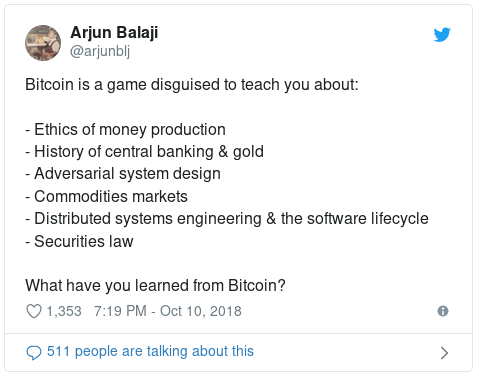
\includegraphics[width=7cm]{assets/images/the-tweet.png}
\end{center}

Die \textit{21 Lektionen} sind in Siebener-Bündel gegliedert, was letztendlich
zu drei Kapiteln führt. Jedes Kapitel betrachtet Bitcoin durch eine
unterschiedliche Linse und zeigt, welche Erkenntnisse daraus gezogen werden
können, wenn man dieses seltsame Netzwerk aus einem anderen Blickwinkel
betrachtet.

\paragraph{\hyperref[ch:philosophy]{Kapitel 1}} untersucht die philosophischen
Lehren von Bitcoin. Das Zusammenspiel von Unveränderlichkeit und Veränderung,
das Konzept der wahren Knappheit, Bitcoins unbefleckte Empfängnis, das Problem
der Identität, der Widerspruch von Replikation und Ort, die Macht der freien
Meinungsäußerung und die Grenzen des Wissens.

\paragraph{\hyperref[ch:economics]{Kapitel 2}} untersucht die wirtschaftlichen
Lehren von Bitcoin. Lektionen über finanzielle Unwissenheit, Inflation, Wert,
Geld und die Geschichte des Geldes, Mindestreserve-Bankensystem und wie Bitcoin
auf raffinierte und kuriose Weise wieder gesundes bzw. solides Geld auf den
Markt bringt.

\paragraph{\hyperref[ch:technology]{Kapitel 3}} untersucht einige der Lehren,
die aus der Auseinandersetzung mit der Technologie von Bitcoin hervorgegangen
sind. Warum es Zahlenstärke gibt, was Vertrauen bedeutet, warum das Messen von
Zeit Arbeit kostet, warum sich langsames Fortbewegen und das Nicht-Aufbrechen
von Dingen ein Funktionsmerkmal und kein Fehler ist, was die Erschaffung von
Bitcoin uns über die Privatsphäre vermitteln kann, warum Cypherpunks Code
schreiben (und nicht Gesetze) und welche Metaphern nützlich sein könnten, um die
Zukunft von Bitcoin zu erforschen.

~

Jede Lektion enthält mehrere Zitate und Links im gesamten Text. Wenn du tiefer
in die Materie eintauchen möchtest, findest du Links zu den wichtigsten
Materialien in den Fußnoten und in den Quellenangaben am Ende des Buches.

Auch wenn einige Vorkenntnisse über Bitcoin von Vorteil sind, hoffe ich, dass
diese Lektionen von jedem interessierten Leser verinnerlicht werden können.
Während einige sich aufeinander beziehen, sollte jede Lektion für sich allein
stehen und unabhängig voneinander gelesen werden können. Ich habe mein Bestes
getan, um mich vor Fachjargon zu scheuen, auch wenn einige domänenspezifische
Vokabeln unvermeidlich sind.

Ich hoffe, dass mein Schreiben anderen als Inspiration dient, unter der
Oberfläche zu graben und einige der tieferen Fragen zu untersuchen, die Bitcoin
aufwirft. Meine eigene Inspiration kam von einer Vielzahl von Autoren, Bloggern,
und anderen kreativen Köpfen aus dem Internet, welchen ich ewig dankbar bin.

Zu guter Letzt: Mein Ziel beim Schreiben ist es, dich nicht von irgendetwas zu
überzeugen. Mein Ziel ist es, dich zum Nachdenken zu bringen und dir zu zeigen,
dass es bei Bitcoin viel mehr gibt, als man denkt. Ich kann dir gar nicht sagen,
was Bitcoin ist oder was Bitcoin dir beibringen wird. Das musst du selbst
herausfinden.

\begin{quotation}\begin{samepage}
\enquote{Danach gibt es kein Zurück mehr. Du nimmst die blaue Pille --- die
Geschichte endet hier, du wachst in deinem Bett auf und glaubst, was du glauben
willst. Du nimmst die rote Pille\footnote{die \textit{orange} Pille} --- du
bleibst im Wunderland, und ich zeige dir, wie weit der Kaninchenbau reicht.}
\begin{flushright} -- Morpheus
\end{flushright}\end{samepage}\end{quotation}

\begin{figure}
  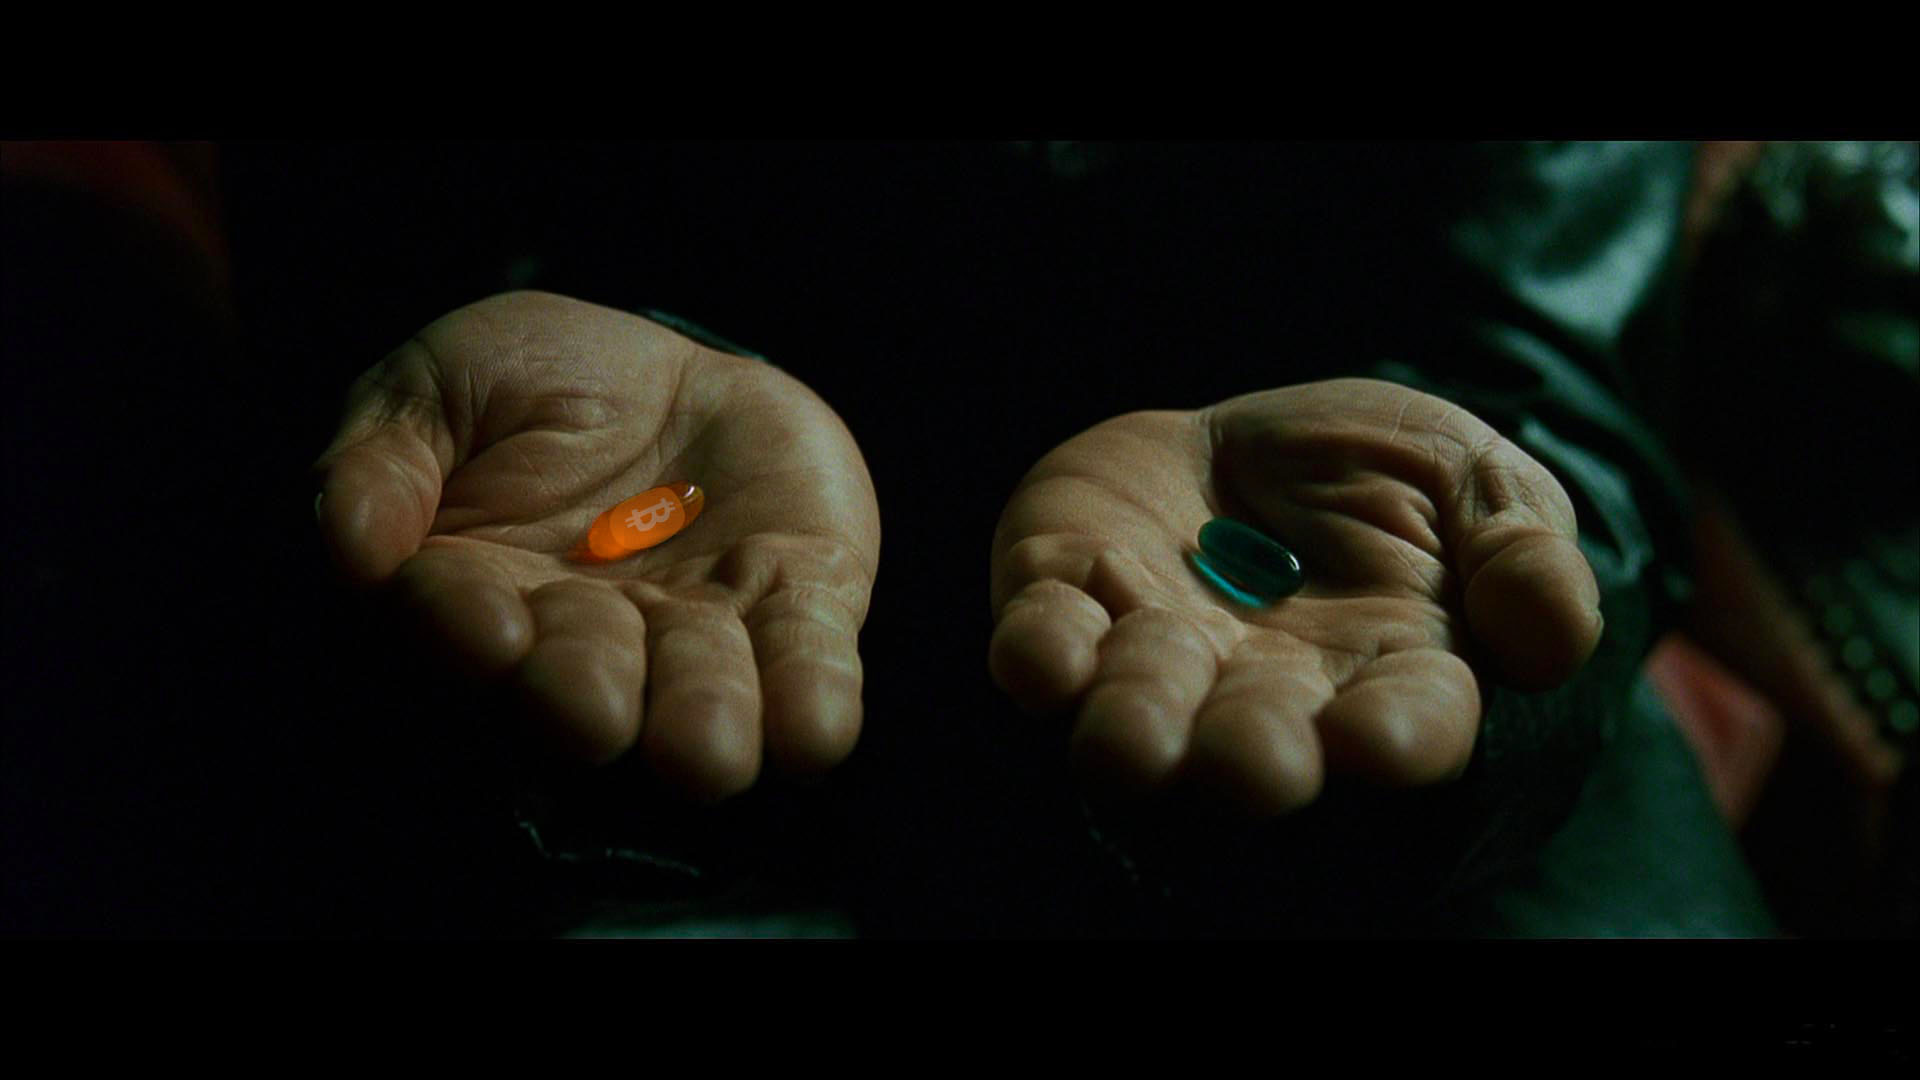
\includegraphics{assets/images/bitcoin-orange-pill.jpg}
  \caption*{Bedenke! Alles, was ich dir anbiete, ist die Wahrheit. Nicht mehr.}
  \label{fig:bitcoin-orange-pill}
\end{figure}

%
% [Morpheus]: https://en.wikipedia.org/wiki/Red_pill_and_blue_pill#The_Matrix_(1999)
% [this question]: https://twitter.com/arjunblj/status/1050073234719293440
%
% <!-- Internal -->
% [chapter1]: {{ 'bitcoin/lessons/ch1-00-philosophy' | absolute_url }}
% [chapter2]: {{ 'bitcoin/lessons/ch2-00-economics' | absolute_url }}
% [chapter3]: {{ 'bitcoin/lessons/ch3-00-technology' | absolute_url }}
%
% <!-- Wikipedia -->
% [alice]: https://en.wikipedia.org/wiki/Alice%27s_Adventures_in_Wonderland
% [carroll]: https://en.wikipedia.org/wiki/Lewis_Carroll
